\chapter{Serie y transformada de Fourier}

Ambas herramientas permiten descomponer una señal en componentes senoidales, revelando su contenido en frecuencia.
Esta perspectiva frecuencial es especialmente útil cuando se analiza el comportamiento de sistemas LIT.
Permite estudiar cómo cada frecuencia es procesada por un sistema de forma independiente.

Las series de Fourier permiten representar funciones \textbf{periódicas} como una suma infinita de exponenciales complejas.
Los coeficientes de los sumandos van a comprender un espectro frecuencial \textbf{discreto} dado por armónicos.

La transformada de Fourier es una transformación lineal que generaliza este concepto hacia señales \textbf{no periódicas}.
Esta herramienta extiende la idea de las series a un espectro frecuencial \textbf{continuo}, mediante integrales en lugar de series.
La transformada inversa permite reconstruir la señal original.

\section{Condiciones de Dirichlet}

La única condición suficiente y necesaria para que la serie de Fourier converja es
\[
    \fx[x]{t} \in \squaredL
\]
osea, que la energía en un período sea finita:
\[
    \int_0^{T_0} \norm{\fx[x]{t}}^2 \dif t < \infty
\]

Por otro lado, las condiciones de Dirichlet son suficientes, pero no necesarias.
Estas son:

\begin{numset}
    \begin{numitem}{Integrabilidad en el período:}
        $\fx[x]{t}$ debe ser absolutamente integrable en un período:
        \[
            \int_{T_0} \norm{\fx[x]{t}} \, \dif t < \infty
        \]
    \end{numitem}

    \begin{numitem}{Número finito de discontinuidades:}
        $\fx[x]{t}$ puede tener en cada período a lo sumo un número finito de discontinuidades de salto finito.
    \end{numitem}

    \begin{numitem}{Número finito de máximos y mínimos:}
        Dentro de un período, $\fx[x]{t}$ debe tener una cantidad finita de máximos y mínimos.
        Es decir, no puede oscilar infinitamente en un intervalo finito.
    \end{numitem}
\end{numset}

\section{Serie de Fourier}

La \emph{serie de Fourier} es una herramienta matemática que permite desarrollar una función periódica (Def. \ref{defn:funcPeriodCont}) como una suma infinita de senos y cosenos armónicos.
Esta descomposición resulta particularmente útil en el análisis de señales, ya que permite estudiar su comportamiento en el dominio de la frecuencia.

Desde un punto de vista matemático, el desarrollo en series de Fourier se basa en la idea de \emph{proyección ortogonal} en un espacio de funciones.
La familia de exponenciales complejas actúa como una base ortonormal.
En este contexto, los coeficientes de la serie se obtienen mediante el \emph{producto interno} entre la señal y cada una de esas funciones base.
A medida que más términos se suman, mejor se aproxima la señal.
La calidad de la aproximación se puede medir mediante el \emph{error cuadrático medio}.
Al proyectar ortogonalmente, este error se minimiza, lo que garantiza que la serie de Fourier es la mejor aproximación posible.

\begin{mdframed}[style=DefinitionFrame]
    \begin{defn}
        \label{defn:FourierSerieExp}
    \end{defn}
    \cusTi{Serie de Fourier: forma exponencial compleja}
    \[
        \fx[x]{t} = \sum_{\kth=-\infty}^\infty c_\kth \, e^{\iu \, \kth \, \omega_0 \, t}
    \]
    \noTi{donde $c_\kth$ son los coeficientes de Fourier complejos, dados por}
    \[
        c_\kth = \frac{1}{T_0} \int_{T_0} \fx[x]{t} \, e^{-\iu \, \kth \, \omega_0 \, t} \, \dif t
    \]
\end{mdframed}

\begin{mdframed}[style=ExampleFrame]
    \begin{example}
    \end{example}
    Determinar la serie de Fourier y el espectro de
    \[
        \fx[x]{t} = 2 + 4 \fx[\cos]{50 t + \frac{\pi}{2}} + 12 \fx[\cos]{100 t - \frac{\pi}{3}}
    \]

    \concept{Resolución}

    A partir de la suma de un complejo con su conjugado, podemos expresar $\fx[x]{t}$ en sumas de exponenciales:
    \begin{align*}
        \fx[x]{t}
        & = 2 + \frac{4}{2} \inBrackets{e^{\iu \inParentheses{50 t + \frac{\pi}{2}}} + e^{- \iu \inParentheses{50 t + \frac{\pi}{2}}}} +
        \notag
        \\
        & \hfill \hspace{2cm}
        + \frac{12}{2} \inBrackets{e^{\iu \inParentheses{100 t - \frac{\pi}{3}}} + e^{- \iu \inParentheses{100 t - \frac{\pi}{3}}}}
        \\[2ex]
        & = 2 + 2 \, e^{\iu \inParentheses{50 t + \frac{\pi}{2}}} + 2 \, e^{\iu \inParentheses{- 50 t - \frac{\pi}{2}}} +
        \notag
        \\
        & \hfill \hspace{2.5cm}
        + 6 \, e^{\iu \inParentheses{100 t - \frac{\pi}{3}}} + 6 \, e^{\iu \inParentheses{- 100 t + \frac{\pi}{3}}}
    \end{align*}

    La frecuencia fundamental es $\omega_0 = \radpers[50]$ luego
    \begin{align*}
        \fx[x]{t}
        & = 2 + 2 \, e^{\iu \frac{\pi}{2}} \, e^{\iu \omega_0 t} + 2 \, e^{- \iu \frac{\pi}{2}} \, e^{- \iu \omega_0 t} +
        \notag
        \\
        & \hfill \hspace{2.5cm}
        + 6 \, e^{- \iu \frac{\pi}{3}} \, e^{\iu 2 \, \omega_0 \, t} + 6 \, e^{\iu \frac{\pi}{3}} \, e^{- \iu 2 \, \omega_0 \, t}
        \\[2ex]
        & = 2 \, e^0 + 2 \iu \, e^{\iu \omega_0 t} - 2 \, \iu \, e^{- \iu \omega_0 t} +
        \\
        & \hfill \hspace{0.5cm}
        + (3 - \iu 3 \sqrt{3}) \, e^{\iu 2 \, \omega_0 \, t} + (3 + \iu 3 \sqrt{3}) \, e^{- \iu 2 \, \omega_0 \, t}
    \end{align*}

    Y el espectro es
    \begin{center}
        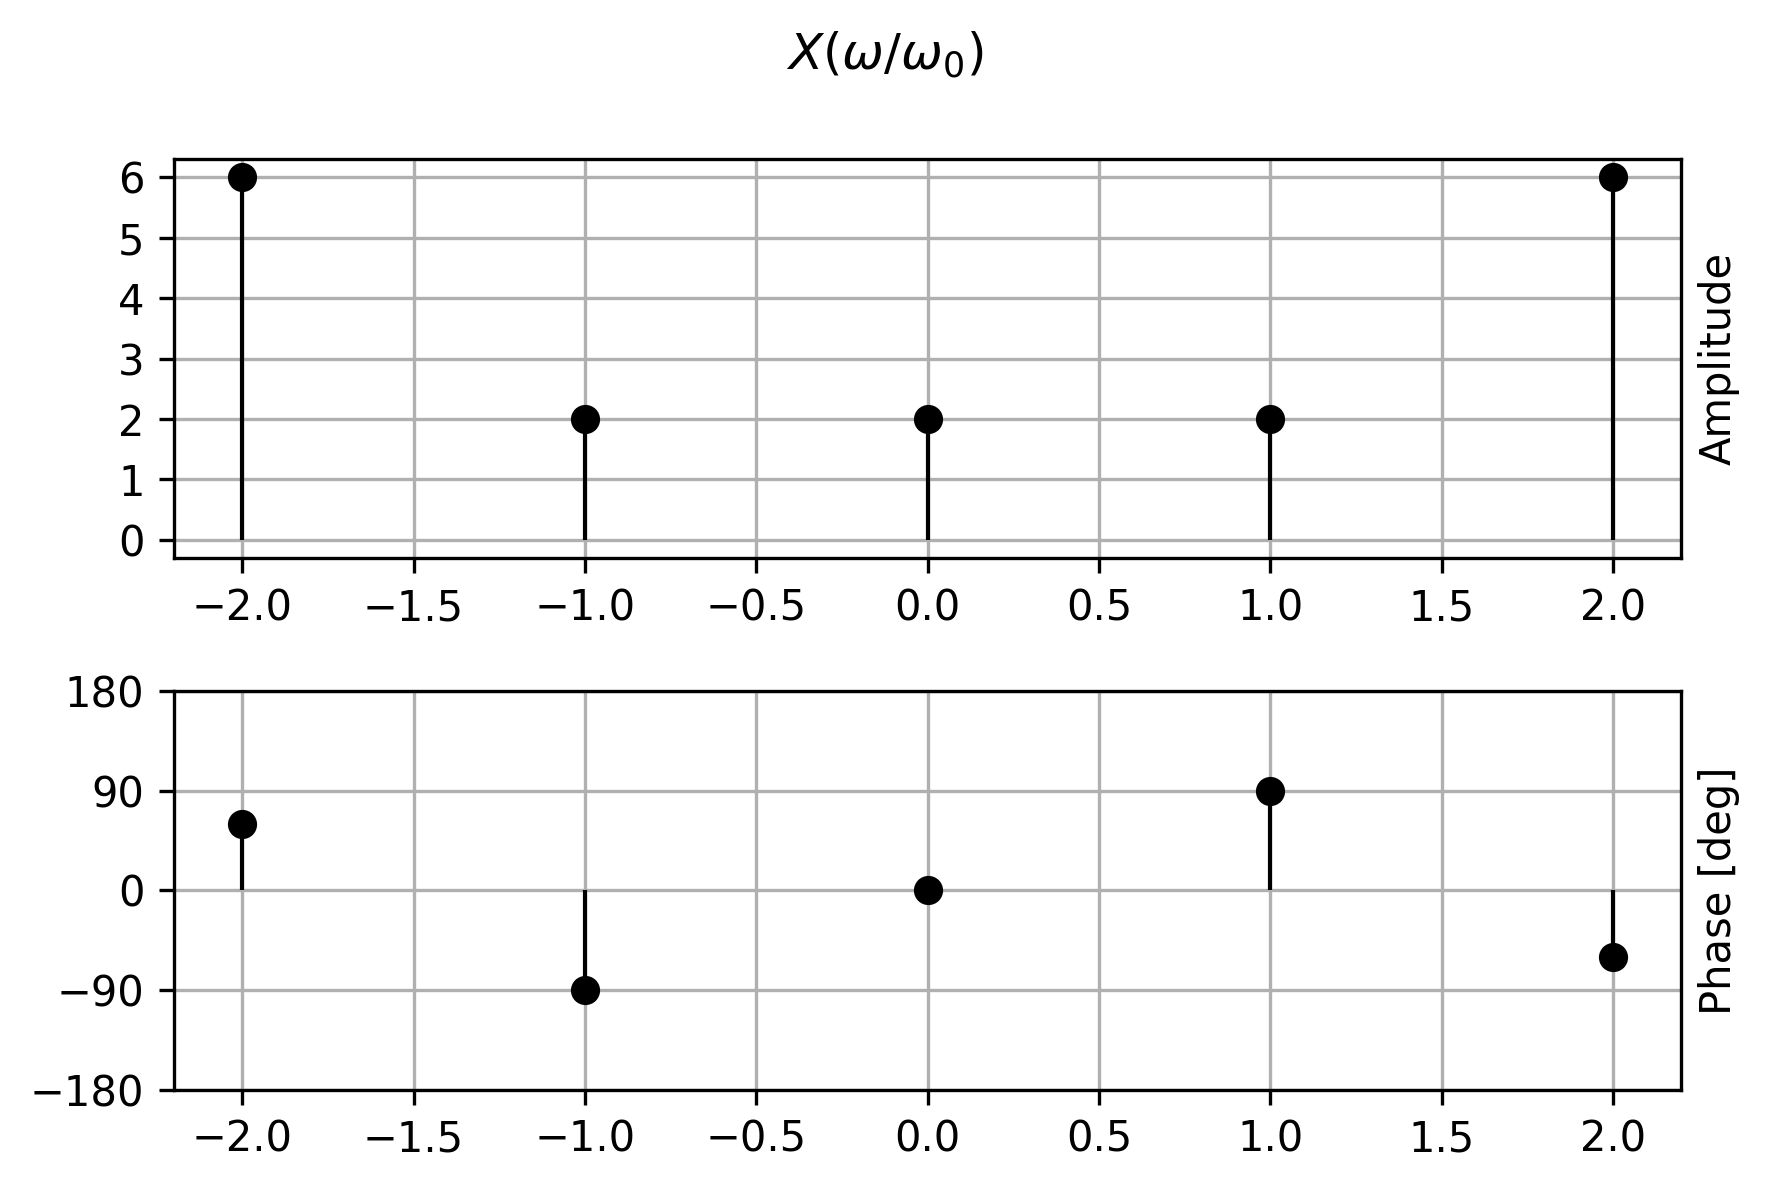
\includegraphics[width=\linewidth]{./images/ej_serie_fourier.png}
    \end{center}
\end{mdframed}

Reacomodando la sumatoria de la definición \ref{defn:FourierSerieExp} según
\begin{align*}
    \fx[x]{t} &=
    \sum_{\kth=-\infty}^\infty c_\kth \, e^{\iu \, \kth \, \omega_0 \, t}
    \\[1em]
    &= \sum_{\kth=-\infty}^{-1} c_\kth \, e^{\iu \, \kth \, \omega_0 \, t} + c_0 + \sum_{\kth=1}^{\infty} c_\kth \, e^{\iu \, \kth \, \omega_0 \, t}
    \\[1em]
    &= \sum_{\kth=1}^{\infty} c_{-\kth} \, e^{-\iu \, \kth \, \omega_0 \, t} + c_0 + \sum_{\kth=1}^{\infty} c_\kth \, e^{\iu \, \kth \, \omega_0 \, t}
\end{align*}
es posible obtener la siguiente expresión equivalente:
\begin{equation}
    \fx[x]{t} = c_0 + \sum_{\kth=1}^{\infty} \inParentheses{ c_\kth \, e^{\iu \, \kth \, \omega_0 \, t} + c_{-\kth} \, e^{-\iu \, \kth \, \omega_0 \, t} }
    \label{eqn:FourierExpBis}
\end{equation}

Y aplicando la fórmula de Euler:
\begin{align*}
    &
    \scale{0.80}{
    = c_0 + \sum_{\kth=1}^{\infty} \inBraces{c_\kth \inBrackets{\fx[\cos]{\kth \, \omega_0 \, t} + \iu \fx[\sin]{\kth \, \omega_0 \, t}} + c_{-\kth} \inBrackets{\fx[\cos]{\kth \, \omega_0 \, t} - \iu \fx[\sin]{\kth \, \omega_0 \, t}} }
    }
    \\[1em]
    &= c_0 + \sum_{\kth=1}^{\infty} \inBrackets{ \inParentheses{c_\kth + c_{-\kth}} \fx[\cos]{\kth \, \omega_0 \, t} + \iu \inParentheses{c_\kth - c_{-\kth}} \fx[\sin]{\kth \, \omega_0 \, t} }
\end{align*}

\begin{mdframed}[style=DefinitionFrame]
    \begin{defn}
        \label{defn:FourierSerieTrig}
    \end{defn}
    \cusTi{Serie de Fourier: forma trigonométrica}
    \[
        \fx[x]{t} = c_0 + \sum_{\kth=1}^{\infty} \inBrackets{a_\kth \fx[\cos]{\kth \, \omega_0 \, t} + b_\kth \fx[\sin]{\kth \, \omega_0 \, t} }
    \]
    \noTi{donde $a_\kth = c_\kth + c_{-\kth}$ y $b_\kth = \iu \inParentheses{c_\kth - c_{-\kth}}$ son los coeficientes de Fourier trigonométricos.}
\end{mdframed}

Por otro lado, si se aplica la fórmula de Euler pero esta vez en la exponencial de los coeficientes complejos de la definición \ref{defn:FourierSerieExp}:
\begin{align*}
    c_{\pm\kth} &= \frac{1}{T_0} \int_{T_0} \fx[x]{t} \, e^{\mp \iu \, \kth \, \omega_0 \, t} \, \dif t
    \\
    &= \frac{1}{T_0} \int_{T_0} \fx[x]{t} \inBrackets{ \fx[\cos]{\kth \, \omega_0 \, t} \mp \iu \fx[\sin]{\kth \, \omega_0 \, t} } \, \dif t
    \\
    &= \frac{1}{T_0} \int_{T_0} \fx[x]{t} \fx[\cos]{\kth \, \omega_0 \, t} \dif t
    \mp \frac{\iu}{T_0} \int_{T_0} \fx[x]{t} \fx[\sin]{\kth \, \omega_0 \, t} \dif t
\end{align*}

Se definen los términos $\alpha = \int_{T_0} \fx[x]{t} \fx[\cos]{\kth \, \omega_0 \, t} \dif t$ y $\beta = \int_{T_0} \fx[x]{t} \fx[\sin]{\kth \, \omega_0 \, t} \dif t$ para simplificar la notación, tal que:
\[
     c_{\pm\kth} = \frac{\alpha}{T_0} \mp \iu \frac{\beta}{T_0}
\]

Obteniendo las siguientes expresiones para los coeficientes trigonométricos de la definición \ref{defn:FourierSerieTrig}:
\[
    \left\{
    \begin{aligned}
        a_\kth &= c_\kth + c_{-\kth} = \frac{2 \, \alpha}{T_0}
        \\
        b_\kth &= \iu \inParentheses{c_\kth - c_{-\kth}} = \frac{2 \, \beta}{T_0}
    \end{aligned}
    \right.
\]

Esto no es casualidad y viene dado por una propiedad que sale de sumar complejos conjugados.
Podemos comprobarla gráficamente.
Dado que $a_\kth \in \setR$ y $b_\kth \in \setI$ son ortogonales entre sí, los coeficientes $c_{\pm\kth} \in \setC$ no forman cualquier ángulo, sino que $c_\kth$ es el conjugado de $c_{-\kth}$.
A continuación se muestran con flechas en el plano complejo:

\begin{center}
    \def\svgwidth{0.6\linewidth}
    \input{./images/fourier-abc.pdf_tex}
\end{center}

A partir del gráfico anterior, se define el complejo $C_\kth = a_\kth - \iu \, b_\kth$ representado por un punto en el vértice del triángulo gris.

Luego, multiplicando y dividiendo por $\norm{C_\kth}$ la serie de la definición \ref{defn:FourierSerieTrig} se tiene
\[
    \fx[x]{t} = c_0 + \sum_{\kth=1}^{\infty} \norm{C_\kth} \inBrackets{ \dfrac{a_\kth}{\norm{C_\kth}} \fx[\cos]{\kth \, \omega_0 \, t} + \dfrac{b_\kth}{\norm{C_\kth}} \fx[\sin]{\kth \, \omega_0 \, t} }
\]

Por trigonometría se tiene $\fx[\cos]{\theta_\kth} = a_\kth / \norm{C_\kth}$ mientras que $\fx[\sin]{\theta_\kth} = b_\kth / \norm{C_\kth}$ luego:
\[
    \fx[x]{t} = c_0 + \sum_{\kth=1}^{\infty} \norm{C_\kth} \inBrackets{ \fx[\cos]{\theta_\kth} \fx[\cos]{\kth \, \omega_0 \, t} + \fx[\sin]{\theta_\kth} \fx[\sin]{\kth \, \omega_0 \, t} }
\]

Aplicando $\fx[\cos]{\alpha \pm \beta} = \fx[\cos]{\alpha} \fx[\cos]{\beta} \mp \fx[\sin]{\alpha} \fx[\sin]{\beta}$ se infiere:

\begin{mdframed}[style=DefinitionFrame]
    \begin{defn}
        \label{defn:FourierSerieArm}
    \end{defn}
    \cusTi{Serie de Fourier: forma armónica}
    \[
        \fx[x]{t} = c_0 + \sum_{\kth=1}^{\infty} \norm{C_\kth} \fx[\cos]{\kth \, \omega_0 \, t - \theta_\kth}
    \]
    \noTi{donde $C_\kth$ son los coeficientes de Fourier expresados en forma polar, tal que:}
    \[
    \left\{
    \begin{aligned}
        \norm{C_\kth} = \sqrt{a_\kth^2 + b_\kth^2}
        \\
        \theta_\kth = \fx[\artan]{\frac{b_\kth}{a_\kth}}
    \end{aligned}
    \right.
\]
\end{mdframed}

\section{Coeficientes de Fourier típicos}

\concept{Pulso rectangular}

Para un pulso rectangular genérico
\[
    \fx[x]{t} = A \, \fx[\Pi]{\frac{t-t_0}{\tau}}
\]
los coeficientes están dados, según la definición \ref{defn:FourierSerieExp}, como sigue:
\begin{align*}
    c_\kth &= \frac{1}{T_0} \int_{T_0} \fx[x]{t} \, e^{-\iu \, \kth \, \omega_0 \, t} \, \dif t
    \\[1ex]
    &= \frac{A}{T_0} \int_{-\frac{\tau}{2}}^{\frac{\tau}{2}} e^{-\iu \, \kth \, \omega_0 \, t} \, \dif t
    \\[1ex]
    &= \frac{A}{T_0} \barrow{\dfrac{e^{-\iu \, \kth \, \omega_0 \, t}}{-\iu \, \kth \, \omega_0}}{-\frac{\tau}{2}}{\frac{\tau}{2}}
    \\[1ex]
    &= \frac{A}{-2 \, \pi \, \iu \, \kth } \inParentheses{ e^{ -\iu \, \omega_0 \, \kth \frac{\tau}{2}} - e^{ \iu \, \omega_0 \, \kth \frac{\tau}{2}} }
    \\[1ex]
    &= \frac{A}{\pi \, \kth} \, \fx[\sin]{\frac{\omega_0 \, \kth \, \tau}{2}}
    \\[1ex]
    &= \frac{A}{\pi \, \kth} \, \fx[\sin]{\frac{\pi \, \kth \, \tau}{T_0}}
    \\[1ex]
    &= \frac{A \, \tau}{T_0} \cdot
    \frac{ \fx[\sin]{\dfrac{\pi \, \kth \, \tau}{T_0}} }{ \dfrac{\pi \, \kth \, \tau}{T_0} }
\end{align*}
luego
\begin{equation}
    c_\kth = \frac{A \, \tau}{T_0} \, \fx[\sinc]{\frac{\pi \, \kth \, \tau}{T_0}}
    \label{eqn:ckPulso}
\end{equation}

\begin{mdframed}[style=ExampleFrame]
    \begin{example}
    \end{example}
    \cusTi{De la proyección ortogonal a la serie}
    \begin{formatI}
        Calcular la proyección ortogonal de una onda cuadrada.
        Obtener los coeficientes de Fourier complejos.
        Demostrar que son equivalentes a una serie deducida a partir de la proyección.
    \end{formatI}
    \vspace{1em}
    Sea $x$ una función por partes dada por
    \[
        \fx[x]{t} =
        \left\{
        \begin{matrix}
            0 & \text{si } -\pi < t < -\frac{\pi}{2}
            \\
            1 & \text{si } -\frac{\pi}{2} < t < \frac{\pi}{2}
            \\
            0 & \text{si } \frac{\pi}{2} < t < \pi
        \end{matrix}
        \right.
    \]
    
    Sea $B_S$ una base de polinomios trigonométricos.
    A saber:
    \[
        B_S = \inBraces{1; \fx[\sin]{t}; \fx[\cos]{t}; \fx[\sin]{2t}; \dots; \fx[\sin]{\kth t}; \fx[\cos]{\kth t}}
    \]
    
    De manera que la proyección de $x$ sobre $S$ es:
    \begin{multline*}
        \fx[\proy_S]{x} =
        \\
        = \frac{1}{2} + \frac{2}{\pi} \inBrackets{\fx[\cos]{t} - \dfrac{\fx[\cos]{3t}}{3} + \dfrac{\fx[\cos]{5t}}{5} - \dfrac{\fx[\cos]{7t}}{7} \cdots}
    \end{multline*}

    Y puede ser expresada por la siguiente serie:
    \begin{equation}
        \fx[\proy_S]{x} = \frac{1}{2} + \frac{2}{\pi} \sum_{\kth=1}^\infty \frac{\inParentheses{-1}^{\kth+1}}{2 \, \kth - 1} \, \fx[\cos]{\inParentheses{2 \, \kth -1} t}
        \label{eqn:FourierProy}
    \end{equation}

    Reemplazando $A=1$, $T_0=2\,\pi$, $\tau=\pi$ en la ecuación \ref{eqn:ckPulso} obtenida para los $c_\kth$ de un pulso, queda
    \[
        c_\kth = \frac{ \fx[\sin]{\frac{\kth \, \pi}{2}} }{\kth \, \pi}
    \]

    Según la ecuación \ref{eqn:FourierExpBis} se tiene:
    \begin{align*}
        \fx[x]{t} &= c_0 + \sum_{\kth=1}^{\infty} \inParentheses{ c_\kth \, e^{\iu \, \kth \, \omega_0 \, t} + c_{-\kth} \, e^{-\iu \, \kth \, \omega_0 \, t} }
        \\
        &= c_0 + \sum_{\kth=1}^{\infty} \frac{\fx[\sin]{\frac{\kth \, \pi}{2}}}{\kth \, \pi} \inParentheses{ e^{\iu \, \kth \, \omega_0 \, t} + e^{-\iu \, \kth \, \omega_0 \, t} }
    \end{align*}

    Obteniendo el desarrollo en series de Fourier para una onda cuadrada:
    \[
        \fx[x]{t} = c_0 + 2 \sum_{\kth=1}^{\infty} \frac{\fx[\sin]{\frac{\kth \, \pi}{2}}}{\kth \, \pi} \, \fx[\cos]{\kth \, \omega_0 \, t}
    \]

    Observar que este desarrollo es equivalente a la ecuación \ref{eqn:FourierProy}, ya que $\fx[\sin]{\frac{\kth \, \pi}{2}}$ vale 0 para los $\kth$ pares y $\pm1$ para los $\kth$ impares.
\end{mdframed}

\section{Propiedades de la serie de Fourier}

\begin{mdframed}[style=PropertyFrame]
    \begin{prop}
    \end{prop}
    Los coeficientes $c_\kth^\nth$ de la serie de Fourier de la n-ésima derivada están dados por
    \[
        c_\kth^\nth = c_\kth \cdot \inParentheses{\frac{\iu \, 2 \, \pi \, \kth}{T_0}}^\nth
    \]
\end{mdframed}

\section{La transformada y su inversa}

La transformada de Fourier extiende el concepto de serie de Fourier a funciones no periódicas.
Permite descomponer señales en una superposición \textbf{continua} de exponenciales complejas.

Para inferir la transformada de Fourier de manera intuitiva, es preciso considerar en la definición \ref{defn:FourierSerieExp} el siguiente cambio de variable
\[
    \omega = \kth \, \omega_0
\]
tanto para el desarrollo en serie de Fourier
\begin{equation}
    \fx[x]{t}
    = \sum_{\kth=-\infty}^\infty
    c_\kth \, \complexExp
    \label{eqn:serieFourierOmega}
\end{equation}
como para la expresión de los coeficientes
\[
    c_\kth =
    \frac{1}{T_0}
    \int_{-\frac{T_0}{2}}^{\frac{T_0}{2}} \fx[x]{t} \, e^{- \iu \omega t}
    \, \dif t
\]

Pero queremos contemplar la posibilidad de que la función $\fx[x]{t}$ a desarrollar sea de duración finita, extendible por cero fuera de su dominio, pero sin tener que ser periódica.
Además, $\omega$ debería poder tomar cualquier valor real, mientras que a partir de $k \, \omega_0$ solo es posible obtener los armónicos, que son frecuencias discretas.
Para sortear ambas cuestiones, podemos asumir que el período de $\fx[x]{t}$ es
\[
    T_0 \to \infty
\]

Aplicando este límite, se tiene
\begin{equation}
    \lim_{T_0 \to \infty} c_\kth =
    \frac{\omega_0}{2 \pi}
    \int_{-\infty}^\infty \fx[x]{t} \, e^{- \iu \omega t}
    \, \dif t
    \quad \text{con } \omega_0 \to 0
    \label{eqn:coefFourierOmega}
\end{equation}

Quedando definido el \emph{espectro frecuencial} como el límite de los coeficientes de Fourier escalados

\begin{mdframed}[style=DefinitionFrame]
    \begin{defn}
    \end{defn}
    \cusTi{Espectro frecuencial}
    \[
        \fx[X]{\omega} = \lim_{T_0 \to \infty} T_0 \, c_k
    \]
\end{mdframed}

Su expresión está definida por la transformada de Fourier:

\begin{mdframed}[style=DefinitionFrame]
    \begin{defn}
        \label{defn:FourierTrans}
    \end{defn}
    \cusTi{Transformada de Fourier}
    \[
        \fourier{x}
        = \int_{-\infty}^\infty \fx[x]{t} \, e^{- \iu \omega t} \, \dif t
        = \fx[X]{\omega}
    \]
\end{mdframed}

Al reemplazar la expresión obtenida para los coeficientes de la ecuación \ref{eqn:coefFourierOmega} en el desarrollo en series de Fourier de la ecuación \ref{eqn:serieFourierOmega}, se tiene:
\[
    \fx[x]{t}
    = \sum_{\kth=-\infty}^\infty
    \inBrackets{ \frac{\omega_0}{2 \pi} \int_{-\infty}^{\infty} \fx[x]{\tau} \, e^{- \iu \omega \tau} \, \dif \tau }
    \, \complexExp
    \quad \text{con } \omega_0 \to 0
\]

Cuando $T_0 \to \infty$, el espaciado entre frecuencias $\omega_0 = \frac{2\pi}{T_0}$ tiende a cero.
La suma sobre frecuencias discretas $\omega = k \, \omega_0$ se aproxima a una integral sobre el dominio continuo $\omega \in \setR$.
Y el paso $\omega_0$ juega el papel de $\dif \omega$ en el límite de Riemann, que da origen a la transformada de Fourier inversa.

\begin{mdframed}[style=DefinitionFrame]
    \begin{defn}
        \label{defn:FourierTransInv}
    \end{defn}
    \cusTi{Transformada de Fourier inversa}
    \[
        \ffourier{X}
        = \frac{1}{2 \, \pi} \int_{-\infty}^\infty \fx[X]{\omega} \, \complexExp \, \dif \omega
        = \fx[x]{t}
    \]
\end{mdframed}
